\section{Introduction}
What happens to an agent's belief when we steer its behavior? Activation
steering changes what a model does by adding a vector to its hidden
activations at inference time, with no retraining
\citep{turner2023actadd,rimsky2024caa,zou2023repe}. It is cheap, it needs only
a few contrasting examples, and it is being proposed as a safety tool. The
method is now moving from language models to reinforcement learning (RL)
agents, where it has been used to retarget a policy by editing its activations
\citep{mini2023maze}. Agents differ from language models in one way that
matters here: a recurrent agent in a partially observable world keeps its
belief about the hidden state of the world in the same hidden vector that the
steering edit modifies, and the recurrence carries the edit forward at every
step. An edit aimed at a behavior may therefore land on the belief as well.

The question is hard to answer in a language model, where beliefs have no
ground truth. We therefore build Cogniland, a procedurally generated navigation task
in which the belief is the hidden category of the map, the agent must
integrate evidence about it and carry it across a memory corridor, and its
skills, bridging water and tunnelling rock, can be counted. The belief shows
in the final decision, which of two flags the agent walks into, so belief and
behavior are measured separately, and the reward exposes a wrong belief on
some maps and hides it on others.

We train a recurrent PPO agent with no supervision on the category and study
its hidden state in three steps. First we decode the belief and find that it
is a single direction: a logistic regression on one scalar, the projection of
the state on the difference of class means, matches a non-linear probe on the
full state. Second we show that the direction is causal: one write along it
at the end of the corridor moves the flag decision with a sigmoidal dose
response, while random directions of the same size do nothing. Third we steer
a skill, suppressing bridging or tunnelling with gradient steps on the action
probability, and read the belief. The steering works as intended: the tool is
used less and the agent still reaches a flag on most maps. But when the
suppressed tool is the one the map's category needs, the belief moves toward
the other category and the agent walks to the wrong flag in most lakes
episodes and nearly half of the rocky ones (Figure~\ref{fig:illustration}).
Suppressing the other tool leaves the belief alone.

Side effects of steering have been reported in language models, where steering
vectors generalize unreliably \citep{tan2024reliability} and break safety
alignment \citep{korznikov2025rogue}. For agents that carry beliefs in a
recurrent state the question is almost unstudied. Our contributions are:
\begin{itemize}[leftmargin=1.4em, itemsep=1pt]
\item Cogniland, a partially observable navigation task with a ground-truth
belief and countable skills, and a recurrent agent that solves it from reward
alone.
\item The belief is one direction of the hidden state: a scalar reads it as
well as a non-linear probe, and writing to it controls the final decision
with a graded dose response.
\item Steering a navigation skill corrupts this belief and flips the final
decision while navigation stays mostly intact, a failure mode the return
cannot see on balanced maps.
\item We attribute the corruption to entanglement: behavior and belief are not
separable directions of the hidden state, so steering methods for stateful
agents should be evaluated across all capabilities, not only the targeted one.
\end{itemize}

\begin{figure}[htbp]

    \centering

    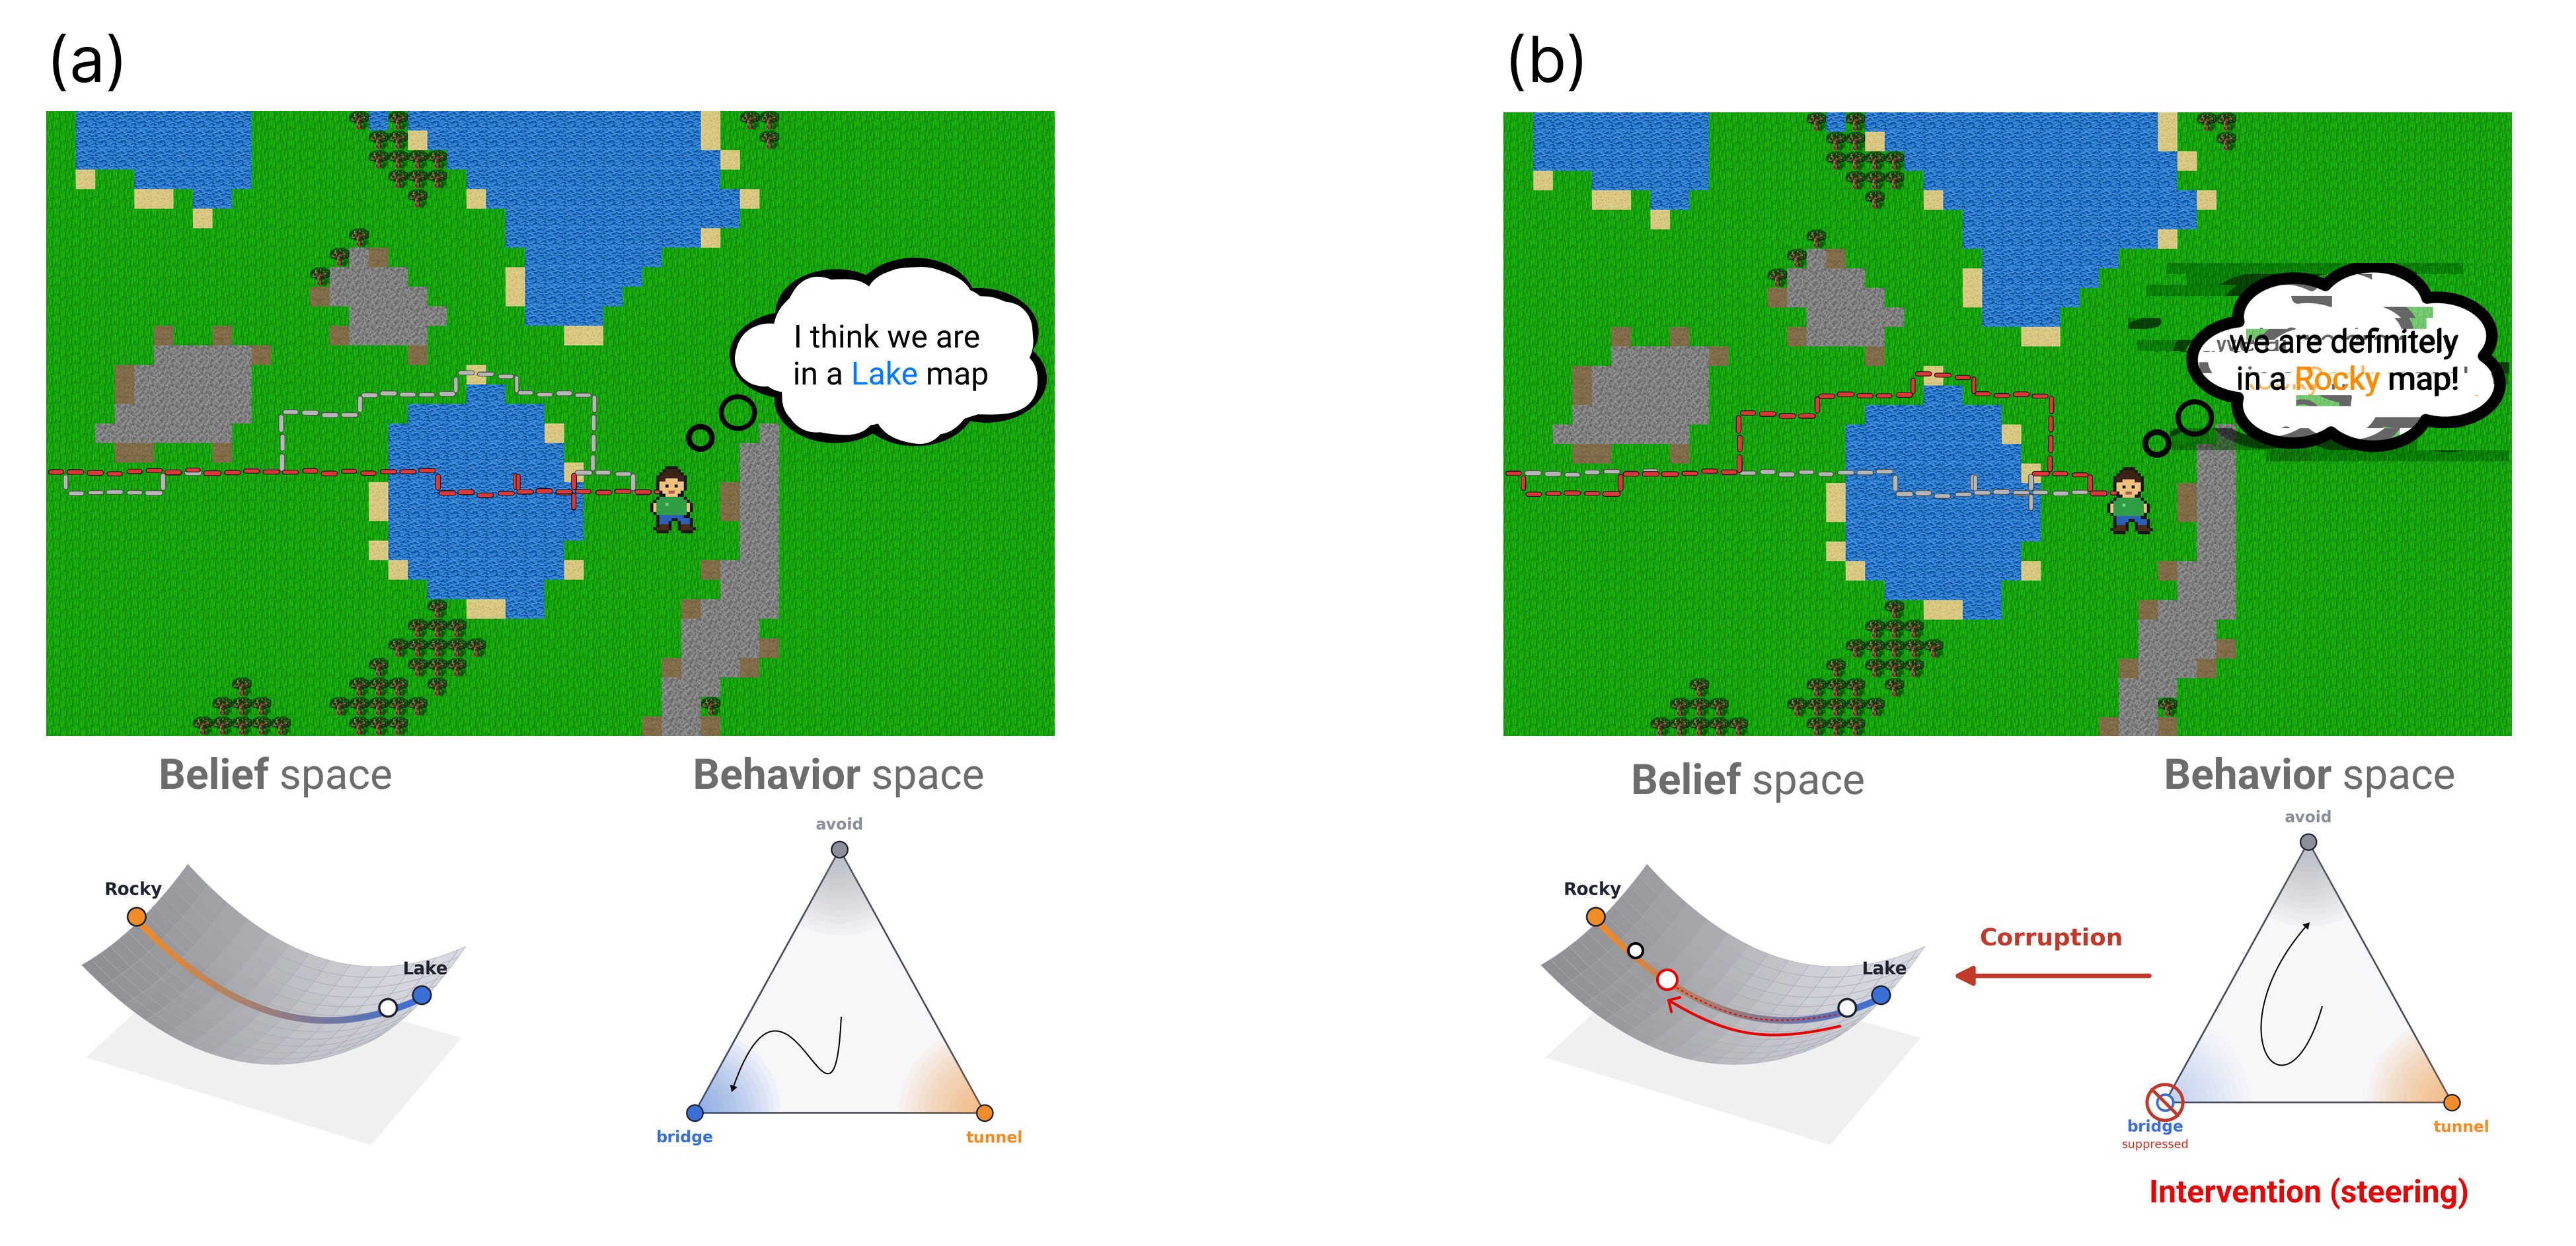
\includegraphics[width=0.95\linewidth]{figures/illustration.png}

    \caption{\textbf{Suppressing a skill corrupts the belief.} Two realizations of an agent deployed on a \textit{lakes} map (a) Unsteered agent: the agent crosses the water by building a bridge, and its belief correctly matches the real category (belief space). (b) Steered agent: bridging is suppressed by activation steering (behavior space): the route changes as intended, but the belief flips towards the wrong category.}
    \label{fig:illustration}

\end{figure}